\documentclass{beamer}

% Chargement du logo
\logo{\includegraphics[height=0.75cm]{images/logo_enseirb.jpg}}

% Choix du thème
\usetheme{CambridgeUS}  % Thème de présentation
\usecolortheme{dolphin} % Thème de couleurs

% Informations sur la présentation
\title{Séance du 24/01}
\author{Projet S8: TRACK}
\institute[T2, Enseirb-Matmeca]{Département Télécommunication\\Enseirb-Matmeca, Bordeaux}
\date{\today}

% Début du document
\begin{document}

% Page de titre
\begin{frame}
  \titlepage
\end{frame}

% Introduction
\begin{frame}
  \frametitle{Ordre du Jour}
  \begin{itemize}
    \item Présentation des avancées
    \item Présentation du calendrier de travail
    \item Questions 
  \end{itemize}
\end{frame}

% Compte rendu des avancées
\begin{frame}
  \frametitle{Compte rendu des avancées}
  \begin{itemize}
    \item MRU :
    \begin{itemize}
        \item[\hspace{1cm}] Théorie implémentée sous Python
        \item[\hspace{1cm}] Premières trajectoires 
    \end{itemize}
    \item MUA
    \begin{itemize}
        \item[\hspace{1cm}] Calculs théoriques réalisés
        \item[\hspace{1cm}] Implémentation sous Python et génération de trajectoire
    \end{itemize}
    \item Singer
    \begin{itemize}
        \item[\hspace{1cm}] Calculs théoriques réalisés
        \item[\hspace{1cm}] Implémentation sous Python et génération de trajectoire
    \end{itemize}
  \end{itemize}
\end{frame}

% Graphiques Trajectoires
\begin{frame}
  \frametitle{Graphiques et Trajectoires : MRU}
  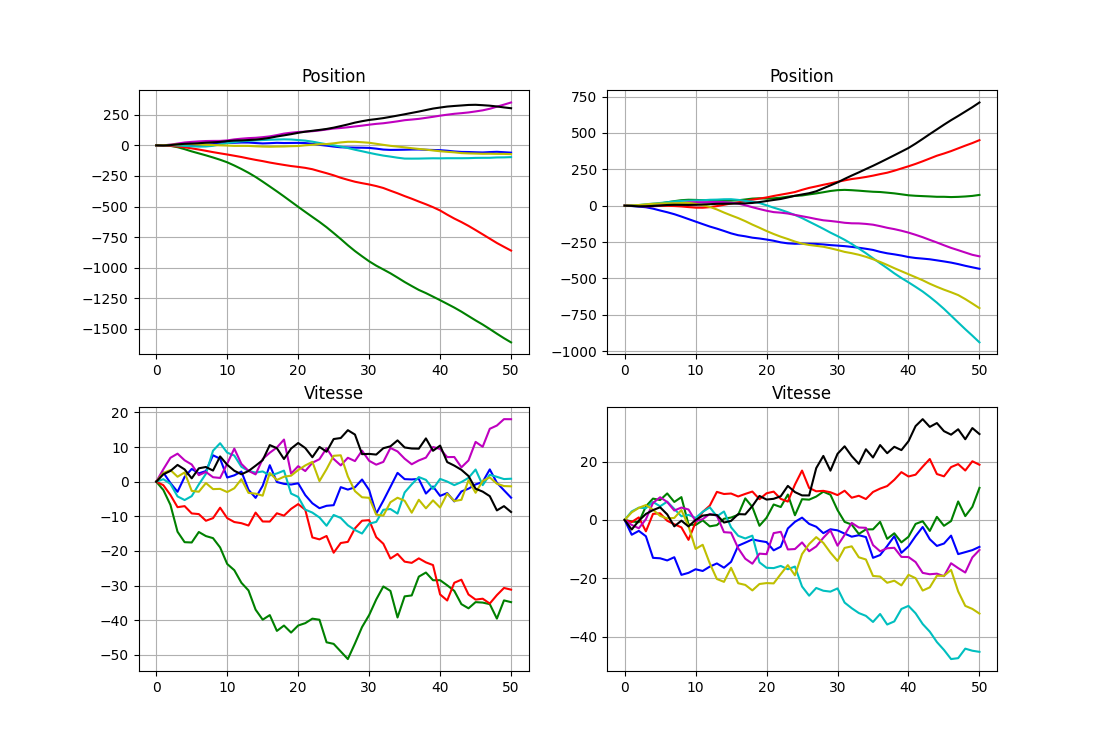
\includegraphics[width=.65\textwidth]{images/MRU_Générations.png}\hfill
  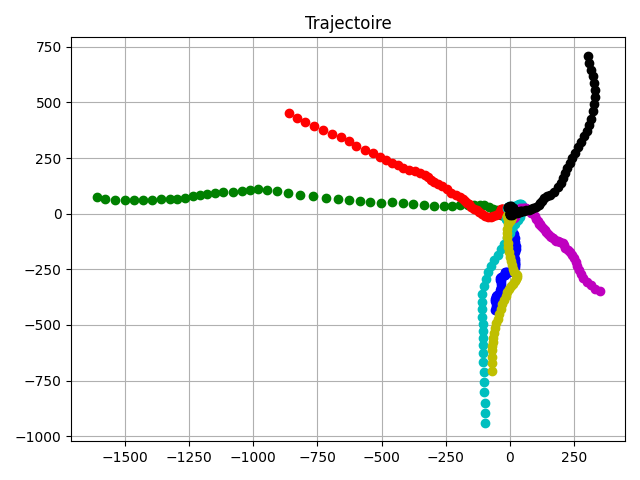
\includegraphics[width=.35\textwidth]{images/MRU_Trajectoires.png} 
  Paramètres : $T_{ech} = 1$, $N = 50$ et $\sigma = 3$
\end{frame}

\begin{frame}
  \frametitle{Graphiques et Trajectoires : MUA}
  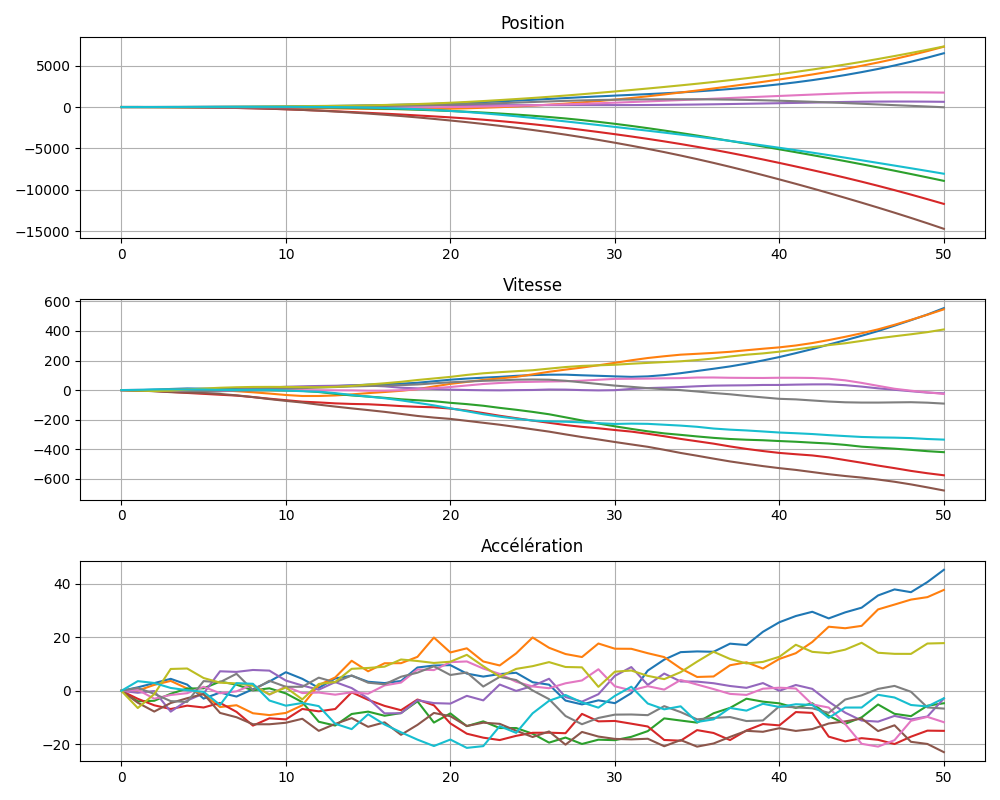
\includegraphics[width=0.75\textwidth]{images/MUA_Générations.png} \\
  Paramètres : $T_{ech} = 1$, $N = 50$ et $\sigma = 3$
\end{frame}

\begin{frame}
  \frametitle{Graphiques et Trajectoires : Singer}
  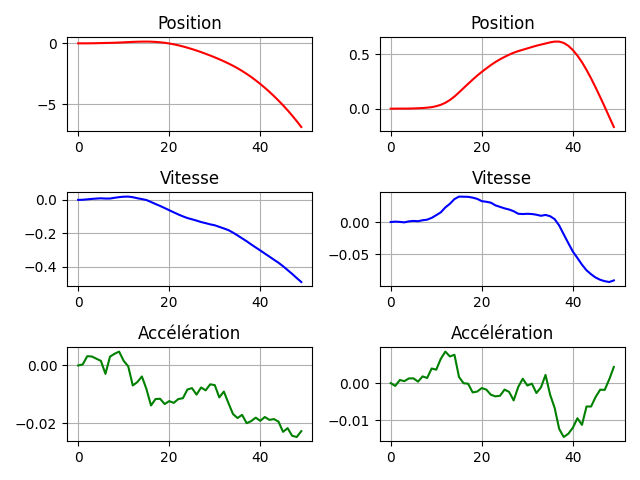
\includegraphics[width=.5\textwidth]{images/SINGER_Générations_1.png}\hfill
  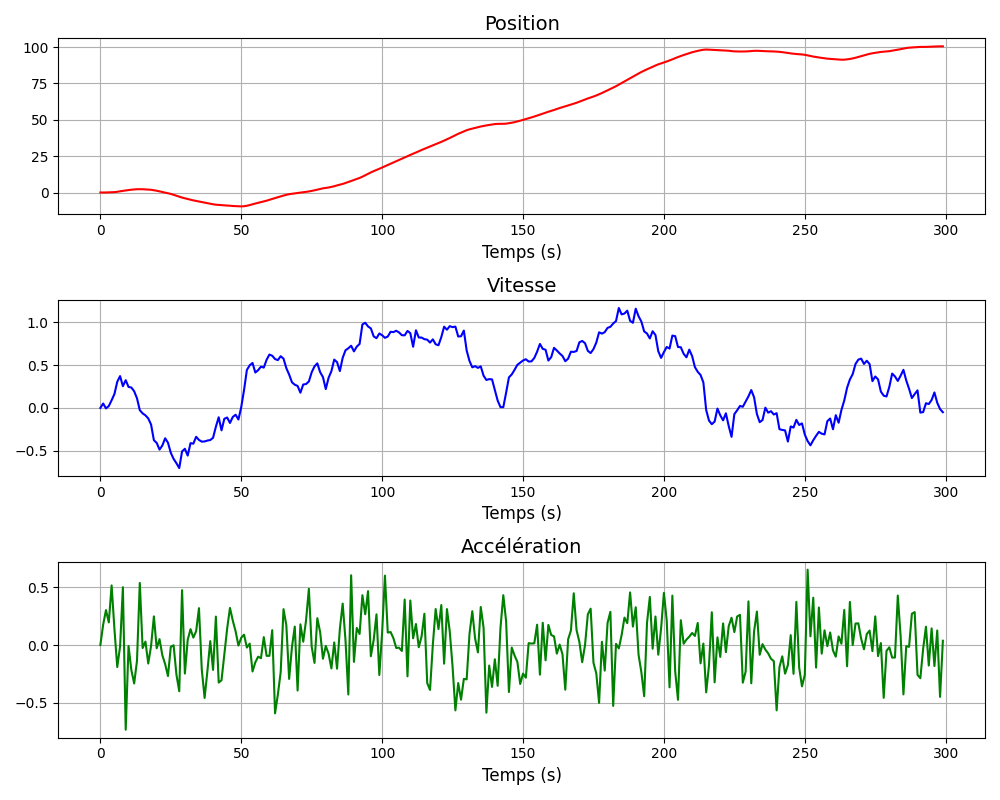
\includegraphics[width=.5\textwidth]{images/SINGER_Générations_2.png} 
  Paramètres : $T_{ech} = 1$, $N = 50$, $\sigma = 3$ et $\alpha = 20$
\end{frame}

% Calendrier de travail
\begin{frame}
  \frametitle{Calendrier de travail}

\end{frame}

% Trello
\begin{frame}{Organisation avec Trello}

  \begin{figure}
      \centering
      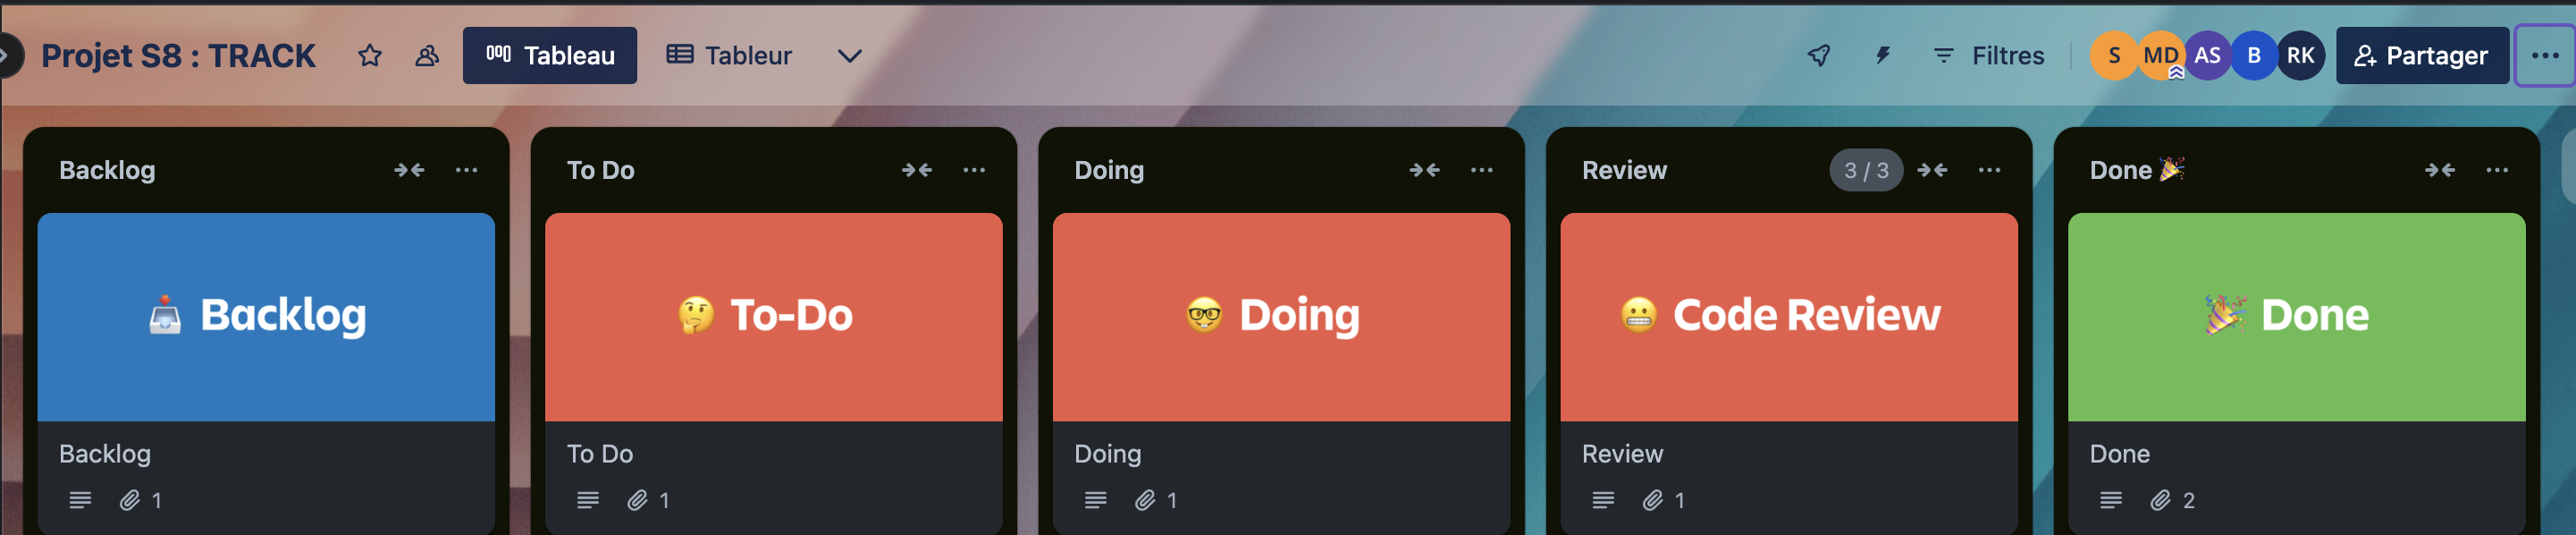
\includegraphics[width=1\linewidth]{images/trello}
      \caption{Capture d'écran de notre espace Trello}
      \label{fig:trello}
  \end{figure}
  
  \begin{itemize}
      \item Division du travail à réaliser en plusieurs tâches grâce à un tableau Kanban, pour assurer un meilleur suivi global.
      \item Organisation du travail selon plusieurs sprints.
  \end{itemize}
  
\end{frame}

% Questions
\begin{frame}
  \frametitle{Questions}
  \begin{itemize}
    \item Cohérence des courbes ?
    \item Quelle quantité d'échantillons ? Tailles variables des échantillons ?
    \item Un format de stockages de donnés à privilégier ? Format initialement choisi : .npy
  \end{itemize}
\end{frame}

% Fin de la présentation
\end{document}
